\section{Reassignment}
\index{asignación}
\index{sentencia!de asignación}
\index{reasignación}


As you may have discovered, it is legal to make more than one assignment to the same variable. A new assignment causes an existing variable to refer to a new value (and no longer refer to the old value).

\begin{Verbatim}[frame=single]
>>> x = 5
>>> x
  5
>>> x = 7
>>> x
  7
\end{Verbatim}
%
The first time we display \texttt{x}, its value is 5; the second time, its value is 7.

Figure~\ref{fig.assign2} shows what a {\bf reassignment} looks like in a state diagram. \index{diagrama!de estado} \index{estado, diagrama de}

\begin{figure}[H]
\begin{center}
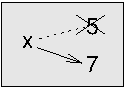
\includegraphics[width=0.25\textwidth]{images/assign2.pdf}
\end{center}
\caption{Reassigning the variable \texttt{x}}
\label{fig.assign2}
\end{figure}

At this point I want to address a common source of confusion. Because Python uses the equals sign (\texttt{=}) for assignment, it is tempting to interpret a statement of the type \texttt{a = b} as a mathematical statement of equality, that is, the statement that \texttt{a} and \texttt{b} are the same. However, this interpretation is incorrect.
\index{igualdad y asignación}

First, equality is a symmetric relation and assignment is not. For example, in math, if $a=7$ then $7=a$. But in Python, the statement \texttt{a = 7} is legal and \texttt{7 = a} is not.

Also, in mathematics, a statement of equality is either true or false all the time. If $a=b$ now, then $a$ will always equal $b$. In Python, an assignment statement can set two variables equal, but they don't have to stay the same:

\begin{Verbatim}[frame=single]
>>> a = 5
>>> b = a    # a and b are equal now
>>> a = 3    # a and b are no longer equal
>>> b
  5
\end{Verbatim}
%
The third line changes the value of \texttt{a} but does not change the value of \texttt{b}, so they are no longer equal.

Variable reassignment is often useful, but you should use it with caution. If the values of the variables change frequently, it can make the code difficult to read and debug.



\hypertarget{update}{%
\section{Variable update}\label{update}}

\index{actualización} \index{variable!actualización}

One of the common uses of assignment statements is to perform an update on a variable -- in which the new value of that variable depends on the old one.

\begin{Verbatim}[frame=single]
x = x + 1
\end{Verbatim}

This means ``take the current value of \texttt{x}, add 1 to it, and then update \texttt{x} with the new value''.

If you try to update a variable that doesn't exist, you'll get an error, since Python evaluates the right hand side before assigning the value to \texttt{x}:

\begin{Verbatim}[frame=single]
>>> x = x + 1
  NameError: name 'x' is not defined
\end{Verbatim}

Before you can update a variable, you must \emph{initialize} it, usually through a simple assignment:

\index{inicialización (antes de actualizar)}

\begin{Verbatim}[frame=single]
>>> x = 0
>>> x = x + 1
\end{Verbatim}

Updating a variable by adding 1 to it is called \emph{incrementing}; subtracting 1 from it is called \emph{decreasing}.

\index{incrementar} \index{decrementar}

\hypertarget{la-instrucción-while}{%
\section{\texorpdfstring{The \texttt{while} statement}{La instrucción while}}\label{la-instrucción-while}}

\index{while, instrucción} \index{instrucción!while} \index{while, bucle}
\index{bucle!while} \index{iteración}

PCs are often used to automate repetitive tasks. Repeating identical or very similar tasks without making mistakes is something that machines are good at and people are not. Because iterations are so common, Python provides several features in its language to make it easier.

One form of iteration in Python is the \texttt{while} statement. Here's a simple program that counts down from five and then says ``Take off!''.

\begin{python}[frame=single]
n = 5
while n > 0:
    print(n)
    n = n - 1
print("Take off!")
\end{python}

It means, ``While \texttt{n} is greater than 0, print the value of \texttt{n} and then reduce the value of \texttt{n} by 1 unit. When you get to 0, exit the \texttt{while} statement and display the expression \texttt{Take off!}''

\index{flujo de ejecución}


The flow of execution of the \texttt{while} statement is represented in Figure \ref{fig:while} and explained in a more formal way as follows:

\begin{enumerate}
\def\labelenumi{\arabic{enumi}.}
\item
  The condition is evaluated, obtaining true or false.
\item
  If the condition is false, the \texttt{while} statement is exited and execution continues at the next statement.
\item
  If the condition is true, the body of the \texttt{while} is executed and then returns to step 1.
\end{enumerate}

\begin{figure}[H]
    \centering
    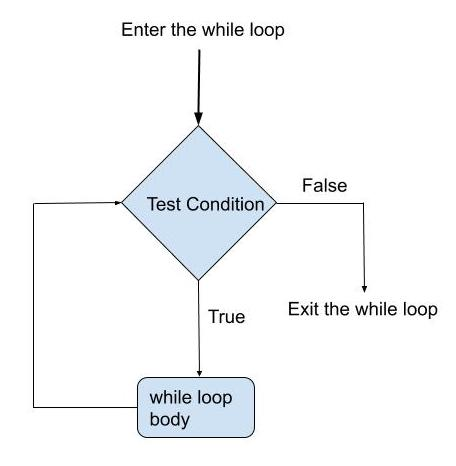
\includegraphics[width=0.50\textwidth]{images/while-eng.jpg}
    \caption{While loop flow}
    \label{fig:while}
\end{figure}

This type of flow is called a \emph{loop}, since the third step links back to the first. Each time the body of the loop is executed we say that we perform an \emph{iteration}. For the loop above, we could say that it ``has had five iterations'', which means that the body of the loop has been executed five times.

\index{condición} \index{bucle} \index{cuerpo}

The body of the loop must change the value of one or more variables, so that the condition may at some point evaluate to false and the loop terminates. The variable that changes each time the loop executes and controls when the loop ends is called the \emph{iteration variable}. If there is no iteration variable, the loop will repeat forever, thus resulting in an \emph{infinite loop}.

To understand how loops work, it's a good idea to make a trace where, for each iteration, we write the values of each of the iteration variables and the results of other actions. For example, consider the following loop:

\begin{python}[frame=single]
i = 1
while (i < 100):
    i = i * 2
    print (i)
\end{python}

An example of a \emph{trace} is in Figure \ref{fig:traza}. We have one column for the condition, one column for each iteration variable, and one more column for the output. It's good practice to do this with your first few loops to understand how they work and to see that the value of the \verb|i| increments each iteration until it has a value greater than 100 so that the loop ends.

\begin{figure}[H]
    \centering
    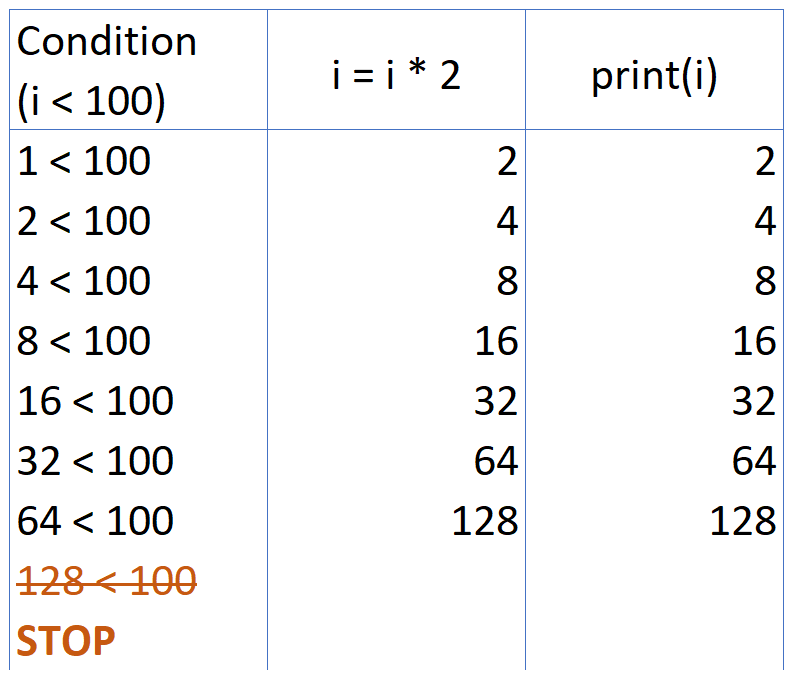
\includegraphics[width=0.4\textwidth]{images/traza-eng.png}
    \caption{Trace the iterations of a loop}
    \label{fig:traza}
\end{figure}


Let's look at another example of a loop:

\begin{python}[frame=single]
while (n != 1):
    print(n)
    if (n % 2) == 0:        #n is even
        n = n / 2
    else:                   #n is odd
        n = n * 3 + 1
\end{python}
%
The condition for this loop is \texttt{(\pythoninline{n} != 1)}, where \pythoninline{n} is the iteration variable. The loop will continue until \pythoninline{n} is \pythoninline{1}, which makes the condition false.

At each iteration through the loop, the program displays the value of \pythoninline{n} and then checks whether it is even or odd. If it is even, \pythoninline{n} is divided by 2. If it is odd, the value of \pythoninline{n} is replaced by \pythoninline{n * 3 + 1}. For example, if the argument passed to \emph{sequence} is 3, the resulting values ​​of \pythoninline{n} are 3, 10, 5, 16, 8, 4, 2, 1.

Since \pythoninline{n} sometimes increases and sometimes decreases, there is no obvious proof that \pythoninline{n} will ever reach 1, or that the program terminates. For some particular values ​​of \pythoninline{n}, we can prove that it terminates. For example, if the initial value is a power of two, \pythoninline{n} will be even each time through the loop until it reaches 1. The above example ends with that sequence, starting with 16.
\index{Collatz, conjetura de}\index{conjetura de Collatz}

The difficult question is whether we can prove that this program terminates for {\em all} positive values of \pythoninline{n}. Until now, no one has been able to prove {\em or} disprove it! (See \url{http://en.wikipedia.org/wiki/Collatz_conjecture})


\begin{exercise}
Trace an execution of the last loop for \pythoninline{(n = 16)}.
\end{exercise}



\hypertarget{bucles-infinitos}{%
\section{Infinite loops}\label{bucles-infinitos}}

An endless source of amusement for programmers is to realise that the shampoo instructions ``Lather, Rinse, Repeat'' are an infinite loop, since there is no \emph{iteration variable} to say how many times the process should be executed.

\index{infinito, bucle} \index{bucle!infinito}

In the case of a \texttt{countdown}, we can verify that the loop terminates, since we know that the value of \texttt{n} is finite, and we can see that the value is getting smaller each time it is counted down. The loop repeats, so at some point it will reach 0. Other times a loop is obviously infinite, because it doesn't have any iteration variables. For example:

\begin{python}[frame=single]
i = 1
while (i < 10):
    print (i)
\end{python}

It's an infinite loop, it will never stop printing the same value of \verb|i|.





\hypertarget{bucles-infinitos-y-break}{%
\section{\texorpdfstring{``Bucles infinitos'' y
\texttt{break}}{``Infinite loops'' and break}}\label{bucles-infinitos-y-break}}

\index{break, sentencia} \index{sentencia!break}

Sometimes you don't know if a loop needs to be terminated until the middle of the loop body has been reached. In that case you can create an infinite loop on purpose and use the \texttt{break} statement to break out of it whenever you want.

The following loop is obviously an \emph{infinite loop}, because the logical expression of the \texttt{while} statement is simply the logical constant \texttt{True}.

\begin{python}[frame=single]
n = 10
while True:
    print(n)
    n = n - 1
print('Finished!')
\end{python}

If you make the mistake of running this code, you'll quickly learn how to stop a stuck Python process on your system, or you'll have to locate where your computer's shutdown button is located. This program will run forever, or until the computer's battery runs out, since the logical expression at the beginning of the loop is always true, by the fact that that expression is precisely the constant value \texttt{True}.

Although it is a useless infinite loop in this case, you can use that design to build useful loops, as long as you take care to add code in the loop body to break out explicitly, using \texttt{break} when the exit condition has been reached.

For example, suppose you want to collect text input from the user until the user types \texttt{end}. You could write:

\pythonexternal[frame=single]{code/copytildone1-eng.py}

The loop condition is \texttt{True}, which is always true, so the loop will repeat until the break statement is executed.

Each time the loop is entered, the user will be prompted for input. If the user types \texttt{finish}, the \texttt{break} statement will break the loop. In any other case, the program will repeat whatever the user types, and will return to the beginning of the loop. This is an example of how it works:

\begin{Verbatim}[frame=single]
> hi everyone
  hola a todos
> I've finished
  I've finished
> finish
  Finished!
\end{Verbatim}

This way of writing \texttt{while} loops is common, since you can check the condition at any point in the loop (not just at the beginning), and you can express the stopping condition affirmatively (``stop when \ldots{} occurs''), instead of having to do it with negative logic (``keep doing it until \ldots{} occurs'').

\hypertarget{finalizar-iteraciones-con-continue}{%
\section{\texorpdfstring{End iterations with \texttt{continue}}{Finalizar iteraciones con continue}}\label{finalizar-iteraciones-con-continue}}

\index{continue, sentencia} \index{sentencia!continue}

Sometimes, being inside a loop, you need to end the current iteration and jump to the next one immediately. In that case, the \texttt{continue} statement can be used to move to the next iteration without terminating the execution of the loop body for the current one.

Here's an example of a loop that repeats what it receives as input until the user types ``end'', but treats lines that start with the hash character as lines that shouldn't be displayed (something like what does Python do with comments?

\pythonexternal[frame=single]{code/copytildone2-eng.py}

Here's an example run of that new program with the \texttt{continue} statement added.

\begin{Verbatim}[frame=single]
> hi everyone
  hi everyone
> # don't print this
> print this!
  print this!
> finish
  Finished!
\end{Verbatim}

All lines are printed to the screen, except the one beginning with the hash symbol, since in that case \texttt{continue} is executed, ending the current iteration, and jumping back to the \texttt{while} statement to begin the next iteration, so that the \texttt{print} statement is skipped.







\hypertarget{bucles-definidos-usando-for}{%
\section{\texorpdfstring{Defined loops using \texttt{for}}{Bucles definidos usando for}}\label{bucles-definidos-usando-for}}

\index{for, sentencia} \index{sentencia!for}

Sometimes you want to loop through a \emph{series} of things, like:

\begin{itemize}[nosep]
    \item a string, for example \verb|"abcdefghijklmnopqrstuvwxyz"|
    \item a list of words, for example \pythoninline{["red", "orange", "yellow", "green"]}
   % \item the lines of a file
    \item a range of values from 1 to 10, for example \pythoninline{range(1,11)}
\end{itemize}
When you have a number of things to loop through, you can build a loop using the \texttt{for} statement with \texttt{in}. The syntax of a \texttt{for} loop is similar to a \texttt{while}, in that there is a \pythoninline{for} statement and a repeating body:

\begin{python}[frame=single]
colours = ["red", "orange", "yellow", "green"]
for colour in colours:
    print('Colours of the rainbow:', colour)
print('Finished!')
\end{python}

In Python terms, the variable \pythoninline{colours} is a four-string list\footnote{We'll examine lists in more detail in a later topic.} and the \texttt{for} loop moves through the list and executes its body once for each of the three strings in the list, producing this output:

\begin{Verbatim}[frame=single]
Colours of the rainbow: red
Colours of the rainbow: orange
Colours of the rainbow: yellow
Colours of the rainbow: green
Finished!
\end{Verbatim}

If you think of colours as a \emph{set}, it would be something like: ``Execute the statements in the body of the loop once \emph{for (for)} each colour that is \emph{in)} the set called colours.''

Reviewing the \texttt{for} loop, \pythoninline{for} and \pythoninline{in} are Python reserved words, while \pythoninline{colour} and \pythoninline{colours} are variables.

Specifically, \pythoninline{colour} is the \emph{iteration variable} for the for loop. The variable \pythoninline{colour} changes for each iteration of the loop and controls when the \texttt{for} loop is terminated. The \emph{iteration variable} loops successively through the four strings stored in the \pythoninline{colours} variable.


The \pythoninline{while} statement is called an \emph{indefinite} loop, because it simply repeats until a certain condition becomes \texttt{False}, while the \pythoninline{for} loop is called a \emph{defined} loop because it iterates through a known set of elements, so it performs as many iterations as there are elements in the set.




\hypertarget{diseuxf1os-de-bucles}{%
\section{Loop designs}\label{diseuxf1os-de-bucles}}

A \texttt{for} or \texttt{while} loop is often used to move through a list of items or the contents of a file and look for something, such as the smallest or largest value of the data we are checking.

Loops are usually built like this:

\begin{itemize}[nosep]
\item
  One or more variables are initialised before the loop starts.
\item
  Some operation is performed on each element in the body of the loop, possibly changing the variables within that body.
\item
  The resulting variables are checked when the loop completes.
\end{itemize}

We will now use a list of numbers to demonstrate the concepts and construction of these loop designs.

\hypertarget{bucles-de-recuento-y-suma}{%
\subsection{Examples: count and add loops}\label{bucles-de-recuento-y-suma}}

For example, to count the number of elements in a list, we can write the following \texttt{for} loop:

\begin{python}[frame=single]
counter = 0
for value in [3, 41, 12, 9, 74, 15]:
    counter = counter + 1
print('Number of elements: ', counter)
\end{python}

We set the variable \texttt{counter} to zero before the loop starts, then write a \texttt{for} loop to move through the list of numbers. Our \emph{iteration} variable is called \texttt{value}, and since we don't use \texttt{value} inside the loop, all it does is control the loop and cause the body of the loop to be executed once for each of the values in the list.

In the body of the loop, we add 1 to the current value of \texttt{counter} for each of the values in the list. While the loop is executing, the value of \texttt{counter} is the number of values that have been seen ``so far''.

After the loop completes, the value of \texttt{counter} is the total number of elements. The total number ``falls into our possession'' at the end of the loop. The loop is constructed so that we get what we want when the loop ends.

Another similar loop, which calculates the total of a set of numbers, is shown below:

\begin{python}[frame=single]
total = 0
for value in [3, 41, 12, 9, 74, 15]:
    total = total + value
print('Total: ', total)
\end{python}

In this loop, we \emph{do} use the \emph{iteration variable}. Instead of simply adding one to \pythoninline{counter} as in the previous loop, now for each iteration of the loop we add the current number (3, 41, 12, etc.) to the current total. If you think of the variable \pythoninline{total}, it contains the ``partial sum of values up to that point''. So before the loop starts, \pythoninline{total} is zero, because no values have been examined yet. During the loop, \pythoninline{total} is the partial sum, and at the end of the loop, \pythoninline{total} is the final total sum of all values in the list.

When the loop executes, \pythoninline{total} accumulates the sum of the elements; a variable used in this way is sometimes called an \emph{accumulator}.

\index{acumulador!sum}

Neither the counting loop nor the sum loop is particularly useful in practice, since there are built-in functions called \pythoninline{len()} and \pythoninline{sum()}, that count the number of elements in a list and the total number of elements in it respectively.

\hypertarget{bucles-de-muxe1ximos-y-muxednimos}{%
\subsection{Maximum and minimum value loops}\label{bucles-de-muxe1ximos-y-muxednimos}}

\index{bucle!máximo} \index{bucle!mínimo} \index{None, valor especial}
\index{valor especial!None}

To find the largest value of a list or sequence, we build the following loop:

\begin{python}[frame=single]
largest = None
print('Value of largest (before):', largest)
for value in [3, 41, 12, 9, 74, 15]:
    if (largest is None) or (value > largest) :
        largest = value
    print('Loop:', value, largest)
print('Value of largest (after):', largest)
\end{python}

When the program runs, you get the following output:

\begin{Verbatim}[frame=single]
Value of largest (before): None
Loop: 3 3
Loop: 41 41
Loop: 12 41
Loop: 9 41
Loop: 74 74
Loop: 15 74
Value of largest (after): 74
\end{Verbatim}

We should think of the variable \pythoninline{largest} as the ``largest value seen so far''. Before the loop, we set \pythoninline{largest} to the value \pythoninline{None}. \pythoninline{None} is a special constant value that can be stored in a variable to indicate that the variable is ``empty''. We need the variable, but we don't know what value to assign to it yet.

Before the loop starts, the largest value seen so far is \pythoninline{None}, since no value has been seen yet. During the execution of the loop, if \pythoninline{highest} is \pythoninline{None}, then we take the first value we have as the largest until then. You can see in the first iteration, when the value of \pythoninline{value} is 3, while \pythoninline{largest} is \pythoninline{None}, we immediately set \pythoninline{largest} to be 3.

After the first iteration, \pythoninline{largest} is no longer \pythoninline{None}, so the second part of the compound logic expression that tests if \pythoninline{value > largest} will fire only when we find a value that is larger than the ``largest up to that point''. When we find a new ``larger'' value, we take that new value for \pythoninline{largest}. You can see in the output of the program that \pythoninline{largest} goes from 3 to 41 and then to 74.

At the end of the loop, all values will have been checked and the \pythoninline{largest} variable will then contain the maximum value in the list.

To calculate the smallest number, the code is very similar with one small change:

\begin{python}[frame=single]
smallest = None
print('Value of smallest (before):', smallest)
for value in [3, 41, 12, 9, 74, 15]:
    if (smallest is None) or (value < smallest):
        smallest = value
    print('Loop:', value, smallest)
print('Value of smallest (after):', smallest)
\end{python}

Again, \pythoninline{smallest} is the ``smallest so far'' before, during, and after the loop execution. When the loop is complete, \pythoninline{smallest} will contain the minimum value of the list.

Also as in the case of the number of elements and the sum, the internal functions \pythoninline{max()} and \pythoninline{min()} make writing such loops unnecessary.



\section{Example: Compute square roots with loops}
\label{squareroot}
\index{raiz cuadrada@raíz cuadrada}

Loops are often used in programs that compute numerical results by starting with an approximate answer and iteratively improving it.
\index{metodo@método!de Newton}

For example, one way to calculate square roots is Newton's method. Suppose you want to know the square root of $a$. If you start with almost any estimate, $x$, you can calculate a best estimate with the following formula:

\[ y = \frac{x + a/x}{2} \]
%
For example, if $a$ is 4 and $x$ is 3:

\begin{Verbatim}[frame=single]
>>> a = 4
>>> x = 3
>>> y = (x + a/x) / 2
>>> y
  2.16666666667
\end{Verbatim}
%
The result is closer to the correct answer ($\sqrt{4} = 2$). If we repeat the process with a new estimate value, it gets even closer:

\begin{Verbatim}[frame=single]
>>> x = y
>>> y = (x + a/x) / 2
>>> y
  2.00641025641
\end{Verbatim}
%
After a few more updates, the estimate is almost exact:
\index{actualizar}

\begin{Verbatim}[frame=single]
>>> x = y
>>> y = (x + a/x) / 2
>>> y
  2.00001024003
>>> x = y
>>> y = (x + a/x) / 2
>>> y
  2.00000000003
\end{Verbatim}
%
In general, we don't know in advance how many steps it takes to get to the correct answer, but we know when we get it because the estimate stops changing:

\begin{Verbatim}[frame=single]
>>> x = y
>>> y = (x + a/x) / 2
>>> y
  2.0
>>> x = y
>>> y = (x + a/x) / 2
>>> y
  2.0
\end{Verbatim}
%
When \texttt{y == x}, we can stop. Here's a loop that starts with an initial estimate, \texttt{x}, and improves it until it stops changing:

\begin{python}[frame=single]
while True:
    print(x)
    y = (x + a/x) / 2
    if y == x:
        break
    x = y
\end{python}
%
For most values of \texttt{a} this works fine, but in general it is dangerous to test the equality of \texttt{float} numbers. Floating point values are only approximately correct: most rational numbers, such as $1/3$, and irrational numbers, such as $\sqrt{2}$, cannot be exactly represented by a \texttt{float}.
\index{coma flotante}
\index{epsilon}

Instead of checking to see if \texttt{x} and \texttt{y} are exactly the same, it's safer to use the \texttt{abs} function to compute the absolute value, or magnitude, of the difference between them:

\begin{python}[frame=single]
epsilon = 0.0000001
while True:
    print(x)
    y = (x + a/x) / 2
    if (abs(y-x) < epsilon):
        break
    x = y
\end{python}

%
where \pythoninline{epsilon} has a value like \pythoninline{0.0000001} that determines how close is close enough.


\section{Range}\label{depuraciuxf3n}

The \pythoninline{range} function returns an array or sequence of numbers and is therefore useful to use with \pythoninline{for} loops using \pythoninline{in}. For example:

\begin{python}[frame=single]
for i in range(2,5):
    print(i)
\end{python}

\begin{Verbatim}[frame=single]    
>>> %Run
2
3
4
\end{Verbatim}

We see that \pythoninline{range(start, end)} returns the series of integers from \pythoninline{start} to \pythoninline{end}–1.

If we don't specify \pythoninline{start}, the string will start at 0.

\begin{python}[frame=single]
for i in range(4):
    print(i)
\end{python}

\begin{Verbatim}[frame=single]
>>> %Run    
0
1
2
3
\end{Verbatim}

We can also specify an increment between each element of the array with \pythoninline{range(start, end, inc)}. Returns the series of integers from \pythoninline{start} to \pythoninline{end}-1, taking \pythoninline{inc} as increment.

\begin{python}[frame=single]
for i in range(3,12,2):
    print(i)
\end{python}   

\begin{Verbatim}[frame=single]
>>> %Run
3
5
7
9
11
\end{Verbatim}

The increment can be a negative number, to create a series that goes from highest to lowest. For example:

\begin{python}[frame=single]
>>> for i in range(6,1,-1):
    print(i)
\end{python}   

\begin{Verbatim}[frame=single]
>>> %Run
6
5
4
3
2
\end{Verbatim}




\hypertarget{depuraciuxf3n}{%
\section{Debugging}\label{depuraciuxf3n}}

\index{depuración}

As you write larger programs, you may find that you need to spend more and more time debugging them. More code means more opportunities to make a mistake and more places for bugs to hide.

\index{depuración!por bisección} \index{bisección, depuración por}

One method of shortening debugging time is to ``bisection debug''. For example, if there are 100 lines in your program and you check them one at a time, it will take 100 steps.

Instead, try to split the problem in half. Look in the middle of the program, or close to it, for an intermediate value that you can check. Add a \texttt{print} statement (or something else that has a verifiable effect), and run the program.

If at the midpoint the check is wrong, the problem should be in the first half of the program. If this is correct, the problem will be in the second half.

Every time you do a check like this, you halve the number of lines to search. After six steps (which is much less than 100), you'll have it down to a line or two of code, at least in theory.

In practice it is not always clear what ``in the middle of the program'' is, and it is not always possible to place a check there. There is no point in counting the lines and finding the exact midpoint. Instead, think of places in the program where there might be errors and places where it's easy to put a check. Then choose a site where you estimate the chances of the bug being ahead of and behind that check are about the same.

\hypertarget{glosario}{%
\section{Glossary}\label{glosario}}

\begin{description}
\item[accumulator]
A variable used in a loop to add or accumulate a result.
\end{description}

\index{acumulador}

\begin{description}
\item[counter]
A variable used in a loop to count the number of times something happens. We initialise the counter to zero and then increment it each time we want it to ``count'' something.
\end{description}

\index{contador}

\begin{description}
\item[decrement]
An update that decreases the value of a variable.
\end{description}

\index{decremento}

\begin{description}
\tightlist
\item[increase]
An update that increases the value of a variable (often by one unit).
\end{description}

\index{incremento}

\begin{description}
\item[infinite loop]
A loop in which the termination condition is never satisfied or for which no termination condition exists.
\end{description}

\index{infinito, bucle} \index{bucle!infinito}

\begin{description}
\item[initialise]
An assignment that gives an initial value to a variable that is later to be updated.
\end{description}

\index{inicializar!variable}

\begin{description}
\tightlist
\item[iteration]
Repeated execution of a series of statements using either a function that calls itself or a loop.
\end{description}

\index{iteración}

\section*{Exercises}\label{ejercicios}
\addcontentsline{toc}{section}{Exercises}

\begin{exercise}
What does the following program do? Make a trace.
\pythonexternal[frame=single]{code/ejercicio4_while1.py}
\end{exercise}

\begin{exercise}
What does the following program do? Make a trace.
\pythonexternal[frame=single]{code/ejercicio4_while2.py}
\end{exercise}

\begin{exercise}
What does the following program do? Make a trace.
\pythonexternal[frame=single]{code/ejercicio4_while3.py}
\end{exercise}

\begin{exercise}
What does the following program do? Make a trace.
\pythonexternal[frame=single]{code/ejercicio4_while4-eng.py}
\end{exercise}

\begin{exercise}
What does the following program do? Make a trace.

\pythonexternal[frame=single]{code/ejercicio_for-eng.py}

What will be the result of the program if the data entered are 3 and 6? Why?
What if the data entered were 7 and 7?
Does the output of the program depend on the order in which the data is entered? Why?
Express with a formula what calculation this program does when a <= b.

\end{exercise}


\begin{exercise}

Write a program that repeatedly reads numbers until the user types ``end''. Once ``end'' has been entered, it displays the total, the number of numbers, and the average of those numbers. If the user enters anything other than a number, catch the error using \pythoninline{try} and \pythoninline{except}, then display an error message, and move on to the next number.

Running the program should result in the following:

\begin{Verbatim}[frame=single, label={\em example test execution of the program}]
>>> %Run
  Enter an integer number: 4
  Enter an integer number: 5
  Enter an integer number: wrong data
  Invalid input
  Enter an integer number: 7
  Enter an integer number: end
  16 3 5.33333333333
\end{Verbatim}

Run tests through the console and check the output. Does your program work with negative numbers? Does it work with real numbers? 
\end{exercise}



\begin{exercise}
What does the following program do? Make a trace.

\pythonexternal[frame=single]{code/ejercicio_for1-eng.py}
\end{exercise}

\begin{exercise}
What does the following program do? Make a trace.

\pythonexternal[frame=single]{code/ejercicio_for2.py}
\end{exercise}

\begin{exercise}
What does the following program do? Make a trace.

\pythonexternal[frame=single]{code/ejercicio_for3-eng.py}
\end{exercise}



\begin{exercise}
Implement a program that reads 5 integer and positive numbers and calculates the mean of the numbers and presents it with a maximum of 1 decimal. When the user enters a negative number or another invalid number, you have to ask him again.
 
  Run the following test cases to test your program:

\begin{Verbatim}[frame=single, label={\em test execution of the program}]
>>> %Run 
Enter an integer number: 3
Enter an integer number: 4
Enter an integer number: 0
Enter an integer number: 2
Enter an integer number: 10
The mean of the 5 numbers is 19/5 = 3.8
>>> %Run 
Enter an integer number: -2
Only positive numbers!
Enter an integer number: 2
Enter an integer number: 4
Enter an integer number: r
Invalid input
Enter an integer number: 7
Enter an integer number: 10
Enter an integer number: 0
The mean of the 5 numbers is 23/5 = 4.6
\end{Verbatim}


\end{exercise}

\begin{exercise} 
Write a program that receives an integer $M$ and generates all the numbers that are multiples of 3 between 1 and $M$. Run the following test cases to test your program:

\begin{Verbatim}[frame=single, label={\em test execution of the program}]
>>> %Run 
Enter an integer number: 2
There are no multiples of 3.
>>> %Run 
Enter an integer number: 3
3
>>> %Run 
Enter an integer number: -1
There are no multiples of 3.
>>> %Run 
Enter an integer number: -8
-3,-6
>>> %Run 
Enter an integer number: 30
3,6,9,12,15,18,21,24,27,30
>>> %Run 
Enter an integer number: r
Invalid input
Enter an integer number: hi
Invalid input
Enter an integer number: 10
3,6,9
\end{Verbatim}
\end{exercise}

\begin{exercise} 
Modify the above program so that it displays only those multiples of 3 between 1 and $M$ that are not divisible by 2. Run the following test cases to test your program:

\begin{tabular}{|l|l|l|l|}
\hline
test case ID  & input & expected output  \\ 
\hline\hline
1 & 0 & There are no multiples of 3\\
2 & 2 & There are no multiples of 3\\
3 & -1 & There are no multiples of 3\\
4 & -22 & -3,-9,-15,-21\\
5 & 21 & 3,9,15,21\\
6 & 66 & 3,9,15,21,27,33,39,45,51,57,63\\
\hline
\end{tabular}
\end{exercise}


\begin{exercise}
Write a program that prints the multiplication table, such as the Pythagorean table (named after Pythagoras (\url{https://en.wikipedia.org/wiki/Pythagoras})). The first row and first column contain the numbers to be multiplied (usually the numbers 1 through 10), and at the intersection of each row and each column is the product of the number in its row times the number in its column.


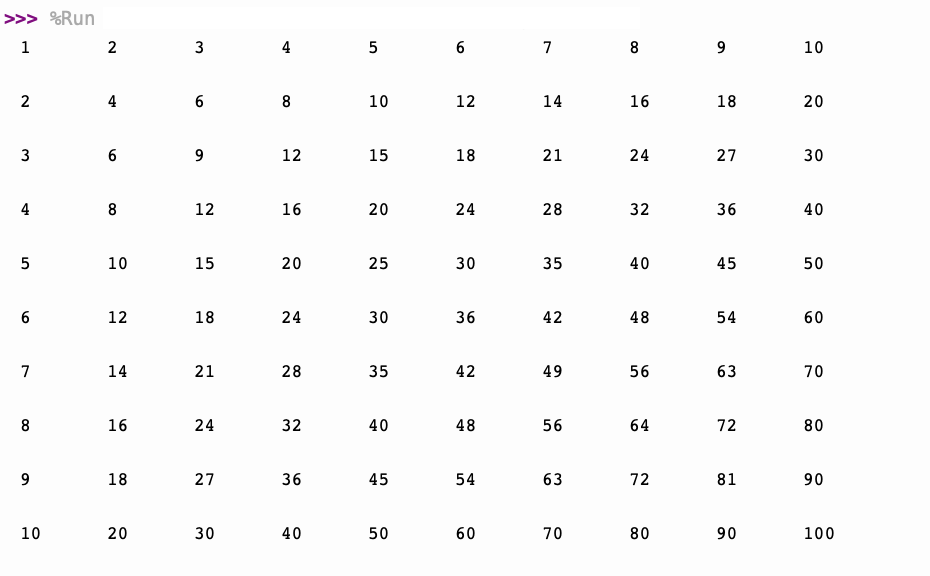
\includegraphics[width=0.75\textwidth]{images/pitagoras.png}
  

\end{exercise}


\begin{exercise}

Write a Python program to print the ASCII values of all characters we have seen using for loop. 

For example, we have seen:

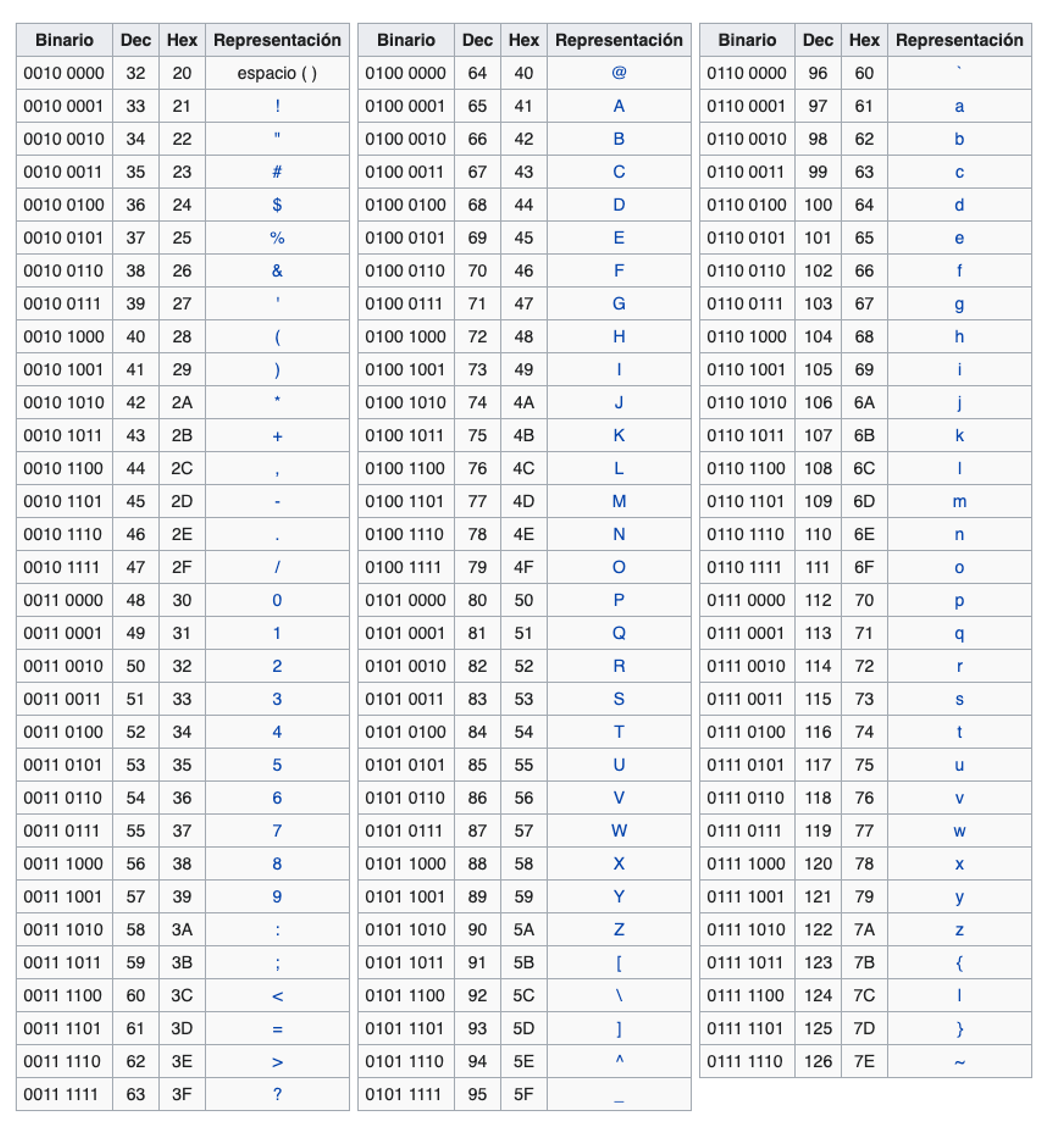
\includegraphics[]{book/Spanish/03_Conditionals_if_elif_else/images/ASCII.png}

\end{exercise}

\begin{exercise}
Strong number is a special number whose sum of factorial of digits is equal to the original number.
For example: 145 is strong number. Since, 1! + 4! + 5! = 145

Write a C program to input number from user and check whether number is Strong number or not. 
\end{exercise}



\section*{Multiple choice exercises}
\addcontentsline{toc}{section}{Multiple choice exercises}

\begin{enumerate}

\item Imagine that we define the following string in Python:

\begin{python}
str = "abcdef"
\end{python}

What comes out when we type?
\begin{python}
for i in range(0, len(str), -1):
        print(str[i])
\end{python}

\begin{choices}
\choice 
\begin{verbatim}
a
b
c
d
e
\end{verbatim}
\choice
\begin{verbatim}
abcde
\end{verbatim}
\choice %CORRECT
\begin{verbatim}

\end{verbatim}
\choice
\begin{verbatim}
fedcba
\end{verbatim}
\end{choices}



\item Imagine that we define the following string in Python:

\begin{python}
str = "abcdef"
\end{python}

What comes out when we type?


\begin{python}
for i in range(-4, 2, 1):
        print(str[i])
\end{python}

\begin{choices}
    \choice %CORRECT
\begin{verbatim}
c
d
e
f
a
b
\end{verbatim}
    \choice
\begin{verbatim}
d
c
b
a
\end{verbatim}
    \choice 
\begin{verbatim}

\end{verbatim}
    \choice
\begin{verbatim}
c
d
e
f
\end{verbatim}
\end{choices}

%\solucion{A.}


\item What comes out when we run the following code?

\begin{python}
i = 0
sum = 0
while i <= 4:
    sum += i
    i = i+1
print(sum)
\end{python}

\begin{choices}
    \choice 10 %CORRECT
    \choice 4
    \choice 5
    \choice 0
\end{choices}

%\solucion{10}



\item Imagine the following statements in Python:


\begin{python}
n = 5
while n > 0:
    if n == 2:
        break
    n = n - 1
    print(n)
print('Loop ended.')
\end{python}

What's the result?

\begin{choices}
    \choice %CORRECT 
\pythoninline{4}\\
\pythoninline{3}\\
\pythoninline{2}\\
\pythoninline{Loop ended.}
    \choice 
\pythoninline{4}\\
\pythoninline{3}\\
\pythoninline{2}\\
\pythoninline{1}\\
\pythoninline{Loop ended.}
    \choice It's an infinite loop
    \choice \pythoninline{NameError: name 'break' is not defined}
\end{choices}

\item Imagine the following statements in Python:


\begin{python}
k = 5
i = -4
while (i <= k):
    i = i + 2
    k = k - 2
    print (i+k)
\end{python}

What's the result?

\begin{choices}
    \choice %CORRECT  
\pythoninline{1}\\
\pythoninline{1}\\
\pythoninline{1}
    \choice 
\pythoninline{2}\\
\pythoninline{3}\\
\pythoninline{4}\\
\pythoninline{5}\\
    \choice 
\pythoninline{3}\\
\pythoninline{3}\\
\pythoninline{3}
    \choice It's an infinite loop

\end{choices}



\item What iterative control structures in Python?

\begin{choices}
    \choice while %choice
    \choice if
    \choice elif
    \choice try
\end{choices}


\item Imagine the following Python program:

\begin{python}
accu = int(input("Enter a value: "))
coun = int(input("Enter another value: "))
prod = 0
vect = 0
while vect > 0: 
    prod = prod + m
    vect += 1 
print("prod is equal to %d." %(prod))
\end{python}

Which option is correct?



\begin{choices}
    \choice prod is an accumulator and vect is a counter %choice
    \choice vect is an accumulator and prod is a counter
    \choice accu is an accumulator and vect is a counter
    \choice accu is an accumulator and coun is a counter
\end{choices}



\end{enumerate}


